% ==================================================================================================================================
% Introduction

\minitoc

Dans ce chapitre, nous allons présenter plus en détail le concept d'ensemble. 
Les ensembles sont les structures les plus primitives des mathématiques, elles permettent par exemple d'effectuer des opérations 
à l'intérieur pour ensuite définir de nouveaux objets plus complexes. 

% ==================================================================================================================================
% Définition et Égalité

\section{Généralités}

\subsection{Définition}

\begin{definition}[Ensemble]
    Un ensemble est une collection non ordonnée d'objets appelés éléments. 
\end{definition}

\textbf{L'ensemble vide}, noté $ \emptyset $, est l’unique ensemble ne contenant aucun élément. 
Un ensemble peut être vu comme un sac contenant divers éléments. 

\begin{example}
    Les entiers positifs constituent un ensemble, de même que les entiers négatifs. 
    On peut aussi parler au sens plus large de l'ensemble des jours de la semaine, ou de l'ensemble 
    des voitures bleues. 
\end{example}

\subsection{Appartenance, Inclusion, Égalité}

La théorie des ensembles est régie par une simple relation : l'appartenance. 

\begin{definition}[Appartenance]
    Soit $E$ un ensemble et $x$ un élément quelconque. 
    On dit que \emph{$x$ appartient à $E$} si $x$ est un élément de $E$. 
    On peut aussi dire que \emph{$E$ contient $x$}. On note alors 
    $x \in E$. 

    Dans le cas contraire, si "$x$ n'est pas dans $E$", on dit que 
    \emph{$x$ n'appartient pas à $E$}. 
    On note alors $x \notin E$. 
\end{definition}

Par extension, on peut définir les notions d'inclusion et d'égalité entre ensembles. 

\begin{definition}[Inclusion]
    Soient $E, F$ deux ensembles. On dit que $F$ est inclus dans $E$ ou que $E$ contient $F$ 
    si tous les éléments de $F$ appartiennent aussi à $E$. On note alors $F \subset E$. 
    Plus formellement, 
        \[ F \subset E \iff \forall x \in F, \; x \in E. \] 
\end{definition}

\begin{definition}[Égalité]
    Soient $E$ et $F$ deux ensembles. On dira qu'ils sont égaux s’ils possèdent 
    exactement les mêmes éléments. On notera alors $E = F$.
    Plus formellement, 
        \[ E = F \iff (\forall x \in E, \; x \in F) \; \text{et} \; (\forall x \in F, \; x \in E). \] 
\end{definition}

\begin{proposition}
    On peut aussi caractériser l'égalité d'ensembles en termes d'inclusions. 
    Ainsi, deux ensembles égaux peuvent aussi être vus comme deux ensembles inclus l'un dans l'autre. 
    D'où : 
        \[ E = F \iff E \subset F \text{ et } F \subset E. \]     
\end{proposition}

Pour montrer une égalité d'ensembles, on utilisera donc préférentiellement le principe de la 
double inclusion. 

% ==================================================================================================================================
% Opérations

\section{Opérations}

Définissons maintenant quelques opérations sur les ensembles. 

\begin{definition}[Opérations]
    Soit $E$ un ensemble et $A$ et $B$ deux parties de $E$. On définit les opérations suivantes : 
    \begin{itemize}
        \item On appelle \textbf{complémentaire} de $A$ dans $E$, noté $\overline{A}$, le sous-ensemble de $E$ 
        qui contient tous les éléments de $E$ qui ne sont pas dans $A$. 
            \[ \overline{A} := \{ x \in E \; | \; x \notin A \}. \] 
        \item On appelle la \textbf{différence} de $A$ par $B$ dans $E$, notée $A \setminus B$, le sous-ensemble de $E$ 
            contenant tous les éléments de $A$ qui ne sont pas dans $B$. 
            \[ A \setminus B := \{ x \in A \; | \; x \notin B \}. \] 
        \item On appelle \textbf{intersection} de $A$ et $B$, notée $A \cap B$, le sous-ensemble de $E$ 
            contenant tous les éléments à la fois dans $A$ \textbf{et} dans $B$. 
                \[ A \cap B := \{ x \in E \; | \; x \in A \text{ et } x \in B \}. \] 
        \item On appelle \textbf{union} de $A$ et $B$, notée $A \cup B$, le sous-ensemble de $E$ 
            contenant tous les éléments appartenant à $A$ \textbf{ou} à $B$. 
                \[ A \cup B := \{ x \in E \; | \; x \in A \text{ ou } x \in B \}. \] 
    \end{itemize}
\end{definition}

\begin{proposition}
    \begin{itemize}
        \item On parlera d'union disjointe de deux ensembles $A$ et $B$ lorsque leur intersection est vide. 
        \item On aura évidemment tout le temps $A \cap B \subset A$ et $A \cap B \subset B$. 
    \end{itemize}
\end{proposition}

\begin{prop}[Opérations]
    Soient $E$ un ensemble et $A, B$ et $C$ des parties de $E$. 
    On a les propriétés suivantes : 
    \begin{enumerate}
        \item Commutativité de $\cap$ et $\cup$ : 
            \[ A \cap B = B \cap A \quad \text{et} \quad A \cup B = B \cup A. \] 
        \item Associativité de $\cap$ et $\cup$ :
            \[ A \cap (B \cap C) = (A \cap B) \cap C \quad \text{et} \quad A \cup (B \cup C) = (A \cup B) \cup C. \] 
        \item Éléments neutres : 
            \[ A \cup \emptyset = A, \quad A \cap E = A, \quad A \cap \emptyset = \emptyset, \quad A \cup E = E. \] 
        \item Distributivité : 
            \[ A \cup (B \cap C) = (A \cup B) \cap (A \cup C) \quad \text{et} \quad A \cap (B \cup C) = (A \cap B) \cup (A \cap C). \] 
        \item Complémentaire involutif : $ \overline{\overline{A}} = A$. 
        \item Lois de De Morgan : 
            \[ \overline{A \cap B} = \overline{A} \cup \overline{B} \quad \text{et} \quad \overline{A \cup B} = \overline{A} \cap \overline{B}. \] 
    \end{enumerate}
\end{prop}



\begin{figure}[h!]
    \centering
    \begin{minipage}{0.45\linewidth}
        \centering
        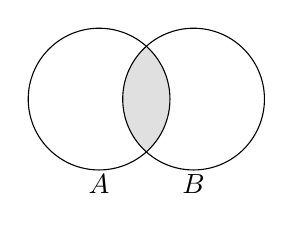
\begin{tikzpicture}[scale=0.6]
            \begin{scope}
                \clip (-1,0) circle (1.5);
                \clip (1,0) circle (1.5);
                \fill[gray!40, opacity=0.6] (-3,-2) rectangle (3,2);
            \end{scope}
            \draw (-1,0) circle (1.5);
            \draw (1,0) circle (1.5);
            \node at (-1,-1.8) {$A$};
            \node at (1,-1.8) {$B$};
        \end{tikzpicture}
        \caption{Union $A \cup B$}
    \end{minipage}
    \hfill
    \begin{minipage}{0.45\linewidth}
        \centering
        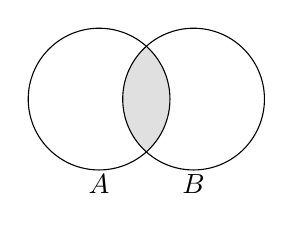
\begin{tikzpicture}[scale=0.6]
            \begin{scope}
                \clip (-1,0) circle (1.5);
                \fill[gray!40, opacity=0.6] (1,0) circle (1.5);
            \end{scope}
            \draw (-1,0) circle (1.5);
            \draw (1,0) circle (1.5);
            \node at (-1,-1.8) {$A$};
            \node at (1,-1.8) {$B$};
        \end{tikzpicture}
        \caption{Intersection $A \cap B$}
    \end{minipage}
\end{figure}

\begin{figure}[h!]
    \centering
    \begin{minipage}{0.45\linewidth}
        \centering
        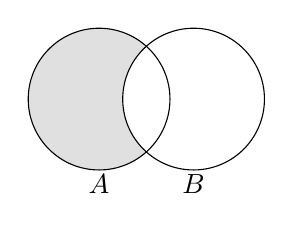
\begin{tikzpicture}[scale=0.6]
            \begin{scope}
                \clip (-1,0) circle (1.5);
                \fill[gray!40, opacity=0.6] (-3,-2) rectangle (3,2);
            \end{scope}
            \begin{scope}
                \clip (-1,0) circle (1.5);
                \fill[white] (1,0) circle (1.5);
            \end{scope}
            \draw (-1,0) circle (1.5);
            \draw (1,0) circle (1.5);
            \node at (-1,-1.8) {$A$};
            \node at (1,-1.8) {$B$};
        \end{tikzpicture}
        \caption{Différence $A \setminus B$}
    \end{minipage}\hfill
    \begin{minipage}{0.45\linewidth}
        \centering
        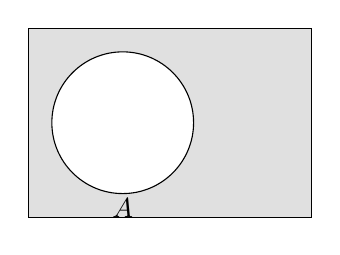
\begin{tikzpicture}[scale=0.6]
            % Univers E
            \fill[gray!40, opacity=0.6] (-3,-2) rectangle (3,2);
            % Ensemble A en blanc
            \fill[white] (-1,0) circle (1.5);
            \draw (-3,-2) rectangle (3,2);
            \draw (-1,0) circle (1.5);
            \node at (-1,-1.8) {$A$};
        \end{tikzpicture}
        \caption{Complémentaire $\overline{A}$}
        \end{minipage}
\end{figure}

\begin{definition}[Produit Cartésien]
    Soient $A$ et $B$ deux ensembles. On définit le produit cartésien de $A$ et $B$, noté $A \times B$, 
    comme l'ensemble composé de tous les couples possibles d'éléments de $A$ et de $B$. 
        \[ A \times B = \{(a,b) \; | \; a \in A, b \in B\} \] 
    Par définition, on dira que $(a,b) \in A \times B$ et $(c,d) \in A \times B$ sont égaux ssi 
    $a = c$ et $b = d$. 
\end{definition}

Par extension, on peut définir le produit cartésien de plusieurs ensembles $A_1, \dots A_n, n \in \N$ 
comme l'ensemble des $n$-uplets de la forme $(a_1, \dots, a_n)$ où tous les $a_i \in A_i, \forall i \in \llbracket 1, n \rrbracket$. 

% ==================================================================================================================================
% Ensemble de nombres

\section{Ensembles de nombres}

En mathématiques, nous travaillons avec différents ensembles de nombres possédant chacun différentes 
propriétés. Il est essentiel de bien les connaître ainsi que leurs relations d'inclusion. 

\subsection{Entiers Naturels}

\begin{definition}[Entiers Naturels]
    L'ensemble des entiers naturels, noté $\N$ est définit par : 
        \[ 0 \in \N \text{ et } \forall n \in \N, n + 1 \in \N \] 
    Autrement dit, $\N$ est le plus petit ensemble contenant $0$ et fermé par l'opération successeur $ : n \mapsto n+1$. 
\end{definition}

On peut aussi définir $\N$ comme l'ensemble $\N := \{1, 2, 3, \dots\}$. Nous choisissons ici d'y inclure $0$. 

\subsection{Entiers Relatifs}

\begin{definition}[Entiers Relatifs]
    On définit l'ensemble des entiers relatifs, noté $\Z$, comme : 
        \[ \Z := \{\dots, -2, -1, 0, 1, 2, \dots\} \]
    Plus formellement, $\Z$ peut être définit comme tous les nombres pouvant être formé de la soustraction 
    de deux entiers naturels. 
        \[ \Z = \{n - m \; | \; n,m \in \N\} \] 
\end{definition}

\begin{proposition}
    Cette définition permet d'en déduire les propriétés suivantes : 
    \begin{itemize}
        \item $\Z$ contient $\N$ 
        \item $\Z$ est fermé par addition et soustraction. 
    \end{itemize}
\end{proposition}

\subsection{Les Rationnels}

\begin{definition}[L'ensemble des Rationnels]
    L'ensemble des rationnels est définit comme l'ensemble des fractions d'entiers relatifs à dénominateur non nul. 
    On le note $\Q$. 
        \[ \Q := \left\{ \frac{a}{b} \; | \; a \in \Z, b \in \Z^* \right\} \] 
\end{definition}

\begin{proposition}
    $\Q$ est fermé par addition, soustraction, multiplication et division (sauf par zéro). 
\end{proposition}

\subsection{Ensemble des nombres réels}

\begin{definition}[Ensemble des nombres réels]
    L'ensemble des nombres réels, noté $\R$, est l'ensemble des limites de suites de rationnels convergentes. 
    On peut aussi le définir comme l'ensemble des nombres pouvant être représentés par une infinité décimale :
    \[
        \R := \text{complétion de } \Q \text{ pour la norme } | \cdot |.
    \]
\end{definition}

\begin{remark}
    \begin{itemize}
        \item $\R$ contient tous les rationnels (\(\Q \subset \R\)) ainsi que tous les nombres irrationnels (comme $\sqrt{2}$, $\pi$).
        \item L'ensemble $\R$ est fermé par addition, soustraction, multiplication et division (sauf par zéro).
        \item Il est ordonné et complet : toute suite croissante et bornée converge dans $\R$.
    \end{itemize}
\end{remark}

\begin{prop}[Inclusions]
    On a toujours les inclusions : 
    \[
        \N \subset \Z \subset \Q \subset \R
    \]
\end{prop}

% ==================================================================================================================================
% Cardinalité d'un ensemble

\section{Cardinalité d'un ensemble}

\begin{definition}[Ensemble fini et Cardinalité]
    Un ensemble $E$ est dit \emph{fini} s'il est vide ou s'il existe un entier naturel $n \in \N$ 
    tel qu'il existe une suite finie d'éléments de $E$, $(x_1, \dots, x_n)$, où chacun de ses éléments 
    apparaît une et une seule fois. 

    Dans ce cas, on dira que $n$ est le \emph{cardinal} de $E$. On le note $|E| = n$.
\end{definition}

\begin{proposition}
    Le cardinal $n \in \N$ d'un ensemble est unique. 
    Le cardinal de l'ensemble vide est 0. 
\end{proposition}

\begin{example}
    \[
        | \{1,2,3\} | = 3, \quad | \emptyset | = 0
    \]
\end{example}

\begin{remark}
    Pour les ensembles infinis (comme $\N$ ou $\R$), on parle de cardinal infini. 
    Deux ensembles $E$ et $F$ ont le même cardinal si une bijection (voir chap. fonctions) existe entre eux.
\end{remark}

\begin{prop}[Cardinal et Opérations]
    Soit $E$ un ensemble fini de cardinal $n \in \N$.
    \begin{itemize}
        \item Tout sous-ensemble de $E$ a un cardinal inférieur ou égal à $n$. 
        \item Si $A$ est un sous-ensemble de $E$ alors $|E/A| = |E|-|A|$. 
        \item Soient $A$ et $B$ deux sous-ensembles de $E$. On a alors : 
            \[ \boxed{| A \cup B = |A| + |B| - | A \cap B |} \] 
    \end{itemize}

\end{prop}
